% Ubah judul dan label berikut sesuai dengan yang diinginkan.
\section{Methodology}
\label{sec:metodologi}

% Ubah paragraf-paragraf pada bagian ini sesuai dengan yang diinginkan.
This research is conducted in accordance with the following system design along with its implementation. The system design is the concept of creating and designing infrastructure, which is then manifested in the form of flow blocks that need to be executed.

In this research, a device integrated with computer vision technology will be developed to control the movement of a wheelchair. Generally, this study will employ a system design as depicted in Figure \ref{fig:Metodologi Penelitian}.

% Gambar 3.1
\begin{figure} [ht] \centering
    % Nama dari file gambar yang diinputkan
    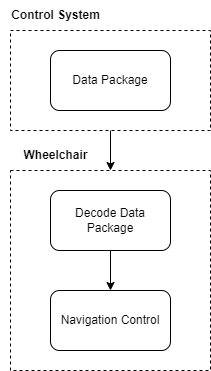
\includegraphics[scale=0.8]{gambar/block diagram.png}
    % Keterangan gambar yang diinputkan
    \caption{Research Block Diagram}
    % Label referensi dari gambar yang diinputkan
    \label{fig:Metodologi Penelitian}
\end{figure}

\subsection{Data Package}
To move the wheelchair, commands need to be sent to the wheelchair controller. In the pose classification phase, basic commands for moving the wheelchair have been obtained, such as forward, backward, right, left, and stop. These commands will then be combined with the maximum speed to form a command or data packet like "Direction, Speed". Direction is a variable with the data type "char" used to control the direction of the wheelchair motor movement. Speed is a variable with the data type "char" used to control the maximum speed of the wheelchair motor rotation.

The direction variable has a "char" data type that determines the movement of the wheelchair motor, while the speed variable has a "char" data type that determines the maximum speed of the wheelchair. To reduce data size, the instruction code to determine the movement direction and maximum speed will be represented by a single letter. The instruction codes can be seen in Table \ref{tbl:kode-instruksi} and Table \ref{tbl:kodePWM}.

After these two variables are combined, they will be sent wirelessly, either using Bluetooth or WiFi, from the laptop or Jetson Nano to the ESP32.
% Tabel 3.2
\begin{table}[h]
  \centering
      \caption{The instruction codes from the pose classification results}
      \label{tbl:kode-instruksi}
      \begin{tabular}{|c|c|}
          \hline
          Pose Classification & Instruction Code \\ \hline
          Left             & A              \\ \hline
          Forward             & B              \\ \hline
          Stop             & C              \\ \hline
          Reverse           & D              \\ \hline
          Right            & E              \\ \hline
      \end{tabular}
\end{table}

\begin{table}[!ht]
    \centering
    \caption{The instruction code for controlling the PWM level}
    \label{tbl:kodePWM}
    \begin{tabular}{|c|c|}
    \hline
    Maximum PWM & Instruction Code \\ \hline
    0           & O                \\ \hline
    31          & P                \\ \hline
    63          & Q                \\ \hline
    95          & R                \\ \hline
    127         & S                \\ \hline
    159         & T                \\ \hline
    191         & U                \\ \hline
    223         & V                \\ \hline
    255         & W                \\ \hline
    \end{tabular}
    \end{table}

After combining both variables, they will be wirelessly transmitted, either using Bluetooth or WiFi, from a laptop or Jetson Nano to the ESP32.

\subsection{Decode Data Package}
The data package sent through the laptop or Jetson Nano will be received by the ESP32 using Bluetooth or WiFi. Upon reception by the ESP32, the data undergoes a series of processes involving data package decoding and adjustment according to the predefined variables. This decoding process allows the ESP32 to decompose the information contained in each package and ensure that each variable is accurately separated. Thus, this process organizes and rearranges the information, ensuring that each variable aligns correctly with the provided variable names and data types.

\subsection{Navigation Control}
Both variables obtained from decoding the data package will be processed on the ESP32. The direction variable will play a role in determining the motor's movement direction, while the speed variable will be used to set the maximum speed of the motor movement. There is a series of chained 'if' logics in the navigation control, where the four direction variables will determine the motor rotation direction. Additionally, the maximum PWM value is configured using the speed variable, allowing users to adjust the maximum motor speed as desired. Thus, at this stage, the ESP32 can effectively process the data received through the wireless system and generate corresponding control instructions to move the wheelchair in the desired direction and speed.